\documentclass{llncs}

\usepackage{amssymb, mathtools, bm}
\usepackage{subfig}
\usepackage{color} 

\DeclareMathOperator{\sgn}{\mathop{sgn}}
\DeclareMathOperator*{\argmin}{arg\,min}
\newcommand{\T}{{\mbox{\scriptsize\sffamily\upshape\mdseries T}}}

\begin{document}
	
\title{Metamodels for Complex Structured Objects Classification}
%
\titlerunning{Metamodels}  % abbreviated title (for running head)
%                                     also used for the TOC unless
%                                     \toctitle is used
%
\author{Roman Isachenko\inst{1} \and Ilya Zharikov\inst{2}
	Artem Bochkarev\inst{3}}
%
\authorrunning{Roman Isachenko et al.} % abbreviated author list (for running head)
%
%%%% list of authors for the TOC (use if author list has to be modified)
\tocauthor{Roman Isachenko, Ilya Zharikov, Artem Bochkarev}
%
\institute{Moscow Institute of Physics and Technology, Institutskiy lane 9, Dolgoprudny, 141700, Russia \\ 
	Skolkovo Institute of Science and Technology, Nobel street 3, Moscow, 143026, Russia\\
	\email{isa-ro@yandex.ru}
	\and
	Moscow Institute of Physics and Technology, Institutskiy lane 9, Dolgoprudny,  141700, Russia \\ 
	Skolkovo Institute of Science and Technology, Nobel street 3, Moscow, 143026, Russia\\
	\email{ilya250894@gmail.com} \and 
	Moscow Institute of Physics and Technology, Institutskiy lane 9, Dolgoprudny, 141700, Russia \\ 
	Skolkovo Institute of Science and Technology, Nobel street 3, Moscow, 143026, Russia\\
	\email{artem.bochkarev@phystech.edu}}

\maketitle              % typeset the title of the contribution

\begin{abstract}
	The development and proliferation of various portable sensors poses new challenges for analyzing and finding meaning in this data. In our work we investigate classification of complex structured objects. One of the main problems in this task is to generate meaningful and relatively small set of features. We compare several approaches for feature extraction such as expertly defined features, autoregressive model and SSA. We propose a new feature generation algorithm, based on local spline approximation. The experiment is conducted on two datasets for human activity recognition using accelerometer.
	\keywords{complex structured objects, time series, local approximation models}
\end{abstract}

\section{Introduction}
This paper investigates the multiclass classification problem of complex structured objects (i.e. we don't have feature representation suitable for direct classification). The application is the human activity recognition. 
The accelerometer time series~\cite{ignatov2016human,lu2016towards,wang2014human} from mobile phones serve to recognize people activity in the internet of things smart homes~\cite{budnik2016learned,lu2016activity}.
New methods in this field range from topological data analysis~\cite{umeda2017time} to convolutional neural networks~\cite{hammerla2016deep}. 
The extensive survey of methods and datasets for this problem is in~\cite{incel2013review}. 

In our work the dataset collects time series of acceleration from three axis, which is obtained from the mobile phone or another wearable device with accelerometer. 
These time series are of different size, not aligned or multiscaled~\cite{geurts2001pattern}.
The problem is to predict physical activity of a person. 
The list of activities includes walking, running, sitting or walking up/down stairs.
In this setup the time series are treated as complex structured objects without explicit feature description. 
This assumption allows to propose a flexible technology of accelerometer time series modelling. 
The main problem to tackle is the lack of computational resources, memory and energy in wearable devices. This investigation proposes an approach to generate features of time series as complex structured objects. The generated features bring adequate quality of classification and require moderate resources.

The problem of classifying complex structured objects is split in two distinctive procedures. 
First, we need to extract informative features, and then we use those features as input to some classifier to obtain final model. 
For simplicity, we assume that these two procedures can be built and analysed separately. 
In our project we focus mainly on comparing different methods of feature generation~\cite{karasikov2016feature,ivkin2015ts}. Existing approaches include expert-defined functions~\cite{kwapisz2011activity}, autoregressive model~\cite{lukashin2003adaptive} and singular spectrum analysis~\cite{hassani2007singular}. 

Expert-defined functions allow to avoid the problem of feature extraction. These functions for time series task include average value, standard deviation, mean absolute deviation and distribution for each component. In autoregressive model we build parametric model for each time series and use parameters of the model as features for classification. Singular spectrum analysis proposes to use eigenvalues of trajectory matrix as features for building classifier.

The experiment was conducted on two accelerometer datasets: WISDM~\cite{wisdm}, USC-HAD~\cite{usc}. 
We compared the performance of stated feature extraction methods, as well as different classification algorithms. 
The latter include logistic regression, random forest and SVM.


\section{Problem Statement}
Let $\mathcal{S}$ be space of complex structured objects, $Y$ is a finite set of class labels. 
We consider accelerometer time series as complex structured objects. Time series is represented as the vector with fixed length $T$:
\begin{equation}
s = [x_1, \dots, x_T]^{\T} \in \mathcal{S}.
\label{eq::time_series}
\end{equation}
We assume that there is a hidden true dependence $f^*: \mathcal{S} \rightarrow Y$ between objects from the space $\mathcal{S}$ and their class labels from $Y$.
Denote by $\mathcal{D} = \{(s_i, y_i)\}_{i=1}^m$ a~given sample, where $s_i \in \mathcal{S}$ and $y_i = f^*(s_i)\in Y$.
The problem is to recover the function~$f^*$. 
We assume that the target function $f^*$ can be approximated by some function $\hat{f}$ from the class of function compositions $f = g \circ \bm{h}$. 
Here $\bm{h}: \mathcal{S} \rightarrow H$ is a map from the original space $\mathcal{S}$ to the feature space $H \subset \bbbr^n$,
$g: H \times \Theta \rightarrow Y$ is a parametric map from the feature space $H$ to the set of class labels $Y$. 
The function $\hat{g}$ corresponds to classification model which is parametrized by a vector parameter $\boldsymbol{\theta} \in \Theta$. 

The determining of the approximation function $\hat{f}$ is equivalent to determining the optimal functions $\bm{h}$ and  $g$. 
The function $\bm{h}$ corresponds to generating the appropriate feature space $H$. 
We consider different local approximation models as the feature generation methods. 
In this case the features are the estimated parameters of the models.

Given appropriate feature space $H$ and feature map $\bm{h}$ we transform our original sample $\mathcal{D} = \{s_i, y_i\}_{i=1}^m$ with complex structured objects to the new sample $\mathcal{D}_H = \{\mathbf{h}_i, y_i\}_{i=1}^m$, where $\mathbf{h}_i = \bm{h}(s_i) \in H$. 
The function $g(\mathbf{h}, \bm{\theta})$ is defined by its parameter vector $\bm{\theta} \in \Theta$. 
The optimal parameters~$\hat{\bm{\theta}}$ are given by
\begin{equation}
\hat{\bm{\theta}} = \argmin_{\bm{\theta}} L(\bm{\theta}, \mathcal{D}_H, \bm{\mu}),
\label{eq::optimal_classification_params}
\end{equation}
where the function $L(\bm{\theta}, \mathcal{D}_H, \bm{\mu})$ is the classification error function. Here the vector $\bm{\mu}$ is a external parameters of the particular classification model. Examples of these parameters for different classification models are given below.

To evaluate the quality of our approximation we consider the accuracy score. 
This choice is based on our wish to compare our results with previous articles~\cite{karasikov2016feature, ivkin2015ts} and easy interpretation. 
Accuracy score is a relation between correctly classified objects and their total number in dataset:
\begin{equation*}
\mathrm{accuracy} = \frac{1}{m} \sum_{i=1}^{m} [y_i = \hat{y}_i],
\end{equation*}
where $\hat{y}_i = \hat{f}(s_i)$ is a prediction of the classifier. 

\section{Feature Generation}

The main focus of this paper is to compare different approaches for feature generation. In this section we provide analysis and motivation behind each of the methods.

\subsubsection{Expert Functions.}

We use the expert-given feature set as the baseline for local approximation models.
These functions are statistics $h_i$, where $h_i: \mathcal{S} \rightarrow \bbbr$.
The description $\bm{h}(s)$ of the object $s$ is the value of these statistics on the object 
\[
\bm{h}(s) = [h_1(s), \dots, h_n(s)]^{\T}.
\]

In paper~\cite{kwapisz2011activity} the authors proposed to use the expert functions listed in table~\ref{tbl::expert_functions}.
This feature generation procedure extracts the feature description of time series $\bm{h}(s) \in \bbbr^{40}$.

\begin{table}[h]
	\centering
	\caption{Expert functions}
	\begin{tabular}{|l|c|}
		\hline
		\textbf{Function description}    & \textbf{Formula} \\ \hline
		Mean                    & $\bar{x} = \frac{1}{T} \sum_{t=1}^{T} x_t$    \\ \hline
		Standard deviation      & $\sqrt{\frac{1}{T} \sum_{t=1}^{T} (x_t - \bar{x})^2}$    \\ \hline
		Mean absolute deviation & $\frac{1}{T} \sum_{t=1}^{T} |x_t - \bar{x}|$    \\ \hline
		Distribution            &  Histogram values with 10 bins    \\ \hline
	\end{tabular}
	\label{tbl::expert_functions}
\end{table}

\subsubsection{Autoregressive Model.}
The autoregressive model~\cite{lukashin2003adaptive} of the order $n$ generates features of time series $s$ with model parameters. 
Each time series is approximated by a linear combination of its previous $n-1$ components 
\begin{equation*}
x_t = w_0 + \sum_{j=1}^{n-1} w_j x_{t-j} + \epsilon_t,
\end{equation*}
where $\epsilon_t$ is a residual. 
The optimal parameters $\mathbf{w}^*$ of the autoregressive model are the features $\bm{h}(s)$.
These parameters minimize the squared error between the time series $s$ and its prediction

\begin{equation}
\bm{h}(s) = \mathbf{w}^* = \argmin_{\mathbf{w} \in \bbbr^{n}} \left( \sum_{t=n}^{T} \|x_t - \hat{x}_t\|^2\right).
\label{eq::autoregressive_description}
\end{equation}
The problem~\eqref{eq::autoregressive_description} is a linear regression problem. Hence, for each initial time series $s$ we have to solve linear regression problem with $n$ predictors.
The example of approximation using autoregressive model is demonstrated on the Fig.~\ref{fig::ar_example}.

\begin{figure}[h]
	\centering
	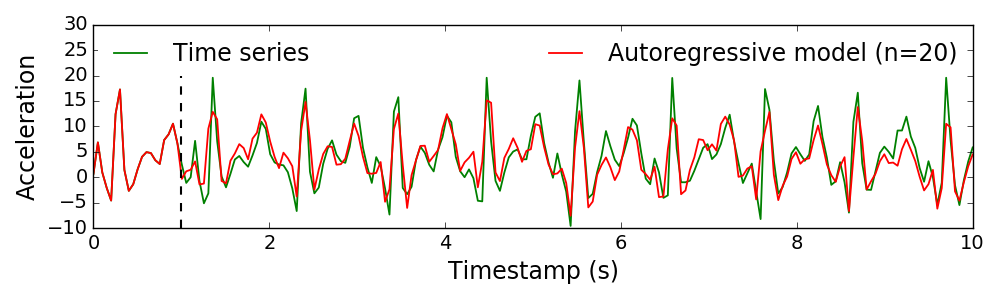
\includegraphics[width=1\linewidth]{pics/ar_example.png}
	\caption{Time series approximation using autoregressive model with order $n = 20$}
	\label{fig::ar_example}
\end{figure}

\subsubsection{Singular Spectrum Decomposition.}
Alternative hypothesis for generation of time series is SSA (Singular Spectrum Analysis) model~\cite{hassani2007singular}. We construct trajectory matrix for each time series $s$ from the original sample $\mathcal{D}$:
\[
\mathbf{X} = 
\begin{pmatrix}
x_1 & x_2 & \dots & x_n \\
x_2 & x_3 & \dots & x_{n+1} \\
\dots & \dots & \dots & \dots \\
x_{T-n+1} & x_{T-n+2} & \dots & x_T
\end{pmatrix}.
\]
Here $n$ is the window width, which is an external structure parameter.
The singular decomposition~\cite{golub1970singular} of the matrix $\mathbf{X}^{\T} \mathbf{X}$:
\[
\mathbf{X}^{\T} \mathbf{X} = \mathbf{U} \mathbf{\Lambda} \mathbf{U}^{\T},
\]
where $\mathbf{U}$ is a unitary matrix and $\Lambda = \mathrm{diag}(\lambda_1, \dots, \lambda_n)$ whose entries $\lambda_i$ are eigenvalues of $\mathbf{X}^{\T} \mathbf{X}$. 
The $n$ largest values of spectrum of the matrix $\mathbf{X}^{\T} \mathbf{X}$ is used as feature description of the object $s$:
\[
\bm{h}(s) = (\lambda_1, \dots, \lambda_n).
\]
\subsubsection{Spline Approximation.}
The proposed method approximates time series with splines~\cite{deboor1978splines}. A spline is defined by its parameters: knots and coefficients.
The set of knots $\{\xi_\ell\}_{\ell=0}^M$ are uniformly distributed over time series.
The models, which are built on each the interval $[\xi_{\ell-1}; \xi_{\ell}]$, are given by the coefficients $\{\mathbf{w}_\ell\}_{\ell=1}^{M}$.

Optimal spline parameters are solution of a system with additional constraints of equality of derivatives up to second order on the edges of intervals. Denote each spline segment as $p_i(t)$ $i = 1, \dots, M$ and spline as a whole as $S(t)$ and write these equations:
\begin{align*}
&S(t) = \begin{cases}
p_1(t) = w_{10} +w_{11}t + w_{12}t^2 + w_{13}t^3, & t\in [\xi_0, \xi_1],\\
p_2(t) = w_{20} +w_{21}t + w_{22}t^2 + w_{23}t^3, & t\in [\xi_1, \xi_2],\\
\cdots &\\
p_{M}(t) = w_{L0} +w_{L1}t + w_{L2}t^2 + w_{L3}t^3, & t\in [\xi_{M-1}, \xi_M],					
\end{cases}\\
&S(t) = x_t \quad t = 1, \dots, T,\\
&p_i'(\xi_i) = p_{i+1}'(\xi_i), \quad p_i''(\xi_i) = p_{i+1}''(\xi_i), \quad i = 1, \dots, M-1.\\
\end{align*}
The feature description of the time series could be assumed as a union of these parameters:
\[
\bm{h}(s) = (\mathbf{w}_1, \dots, \mathbf{w}_{M}).
\]

Fig.~\ref{fig::spline_example} shows the time series approximation given by splines. 
Compared to the autoregressive model, the splines method gives smoother approximation using almost the same number of parameters.

\begin{figure}[h]
	\centering
	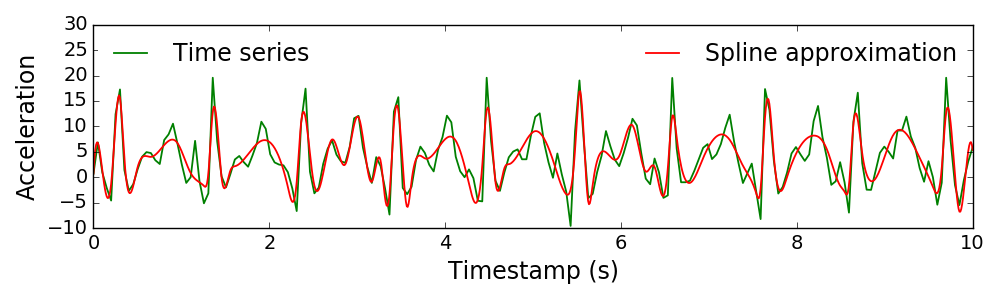
\includegraphics[width=1\linewidth]{pics/spline_example.png}
	\caption{Time series approximation using three order splines}
	\label{fig::spline_example}
\end{figure}

\section{Time Series Classification}
Multiclass classification uses one-vs-rest approach to train binary classifiers for each class label and then, on the prediction step, classify new object according to the most confident classifier. Three classification models are used: logistic regression, SVM and random forest.

\subsubsection{Regularized Logistic Regression.}
The optimal model parameters~\eqref{eq::optimal_classification_params} is determined by minimising the error function

\begin{equation*}
L(\bm{\theta}, \mathcal{D}_H, \mu) = \sum_{i=1}^{m} \log\left(1 + \exp(-y_i [\bm{w}^{\T} \mathbf{h}_i + b])\right) + \frac{\mu}{2} \|\bm{w}\|^2,
\end{equation*}
where 
\begin{equation*}
\bm{\theta}  = \begin{pmatrix}
\bm{w} \\ b
\end{pmatrix}.
\end{equation*}
Thus, 
\begin{equation*}
\bm{\theta}^* = \argmin_{\mathbb{\theta}} L(\bm{\theta}, \mathcal{D}_H, \mu).
\end{equation*}

The classification rule $g(\mathbf{h}, \bm{\theta})$ is given by sign of the linear combination for the object description $\mathbf{h}$ and parameters $\bm{\theta}^*$
\begin{equation*}
\hat{y} = g(\mathbf{h}, \bm{\theta}^*) = \sgn(\mathbf{h}^{\T} \bm{w}^* + b^*).
\end{equation*}

\subsubsection{SVM.}
The problem is

\begin{align*}
\bm{\theta}^*  = \begin{pmatrix}
\bm{w^*} \\ b^* \\ \bm{\xi}^*
\end{pmatrix}= &\argmin_{\bm{w}, b, \bm{\xi}}  \frac{1}{2} \|\bm{w}\|^2 + C\sum_{i=1}^{m} \xi_i,\\
\mbox{subject to} \quad &y_i (\langle \bm{w}, \mathbf{h}_i \rangle + b) \geq 1 - \xi_i,\\
&\xi_i \geq 0, \quad 1 \leq i \leq m.
\end{align*}

The prediction for new object is

\begin{equation*}
\hat{y} = \sgn (\mathbf{h}^{\T} \bm{w}^* + b^*).
\end{equation*}

\subsubsection{Random Forest.}
The random forest exploits the idea of bagging. This is an approach of building many random unstable classifiers and aggregating their predictions. This method works especially well if as base models we select models with low bias and high variance (due to aggregating variance is reduced). In case of random forest decision trees take the role of base models, also not only objects are used for bagging, but also features. In this case we make the prediction for each new object as the mean of the predictions of a single tree:

\begin{equation*}
\hat{y} = \frac{1}{B} \sum_{i=1}^{B} g(\mathbf{h}_i),
\end{equation*}

where $B$ is an amount of trees used for bagging.

\section{Experiment}
In this paper we considered two different smart phone based datasets: WISDM~\cite{wisdm} and USC-HAD~\cite{usc}. 
The smart phone accelerometer measures acceleration along three axis with frequencies equal to 20 and 100 Hz. 
The WISDM dataset consists of 4321 time series. Each time series belongs to one of the six activities: Standing, Walking, Upstairs, Sitting, Jogging, Downstairs. The USC-HAD dataset contains 13620 time series with one of the twelve class labels: Standing, Elevator-up,Walking-forward, Sitting, Walking-downstairs, Sleeping, Elevator-down, Walking-upstairs, Jumping, Walking-right, Walking-left, Running.
The distributions of time series activities for each datasets are presented in table~\ref{tbl::activities_distributions}. 
The length of each time series equals 200 which accounts 10 seconds. 
In the Fig.~\ref{fig::ts_example} the example of the time series for one activity of the specific person is given.

\begin{table}[h]
	\centering
	\caption{Distributions of the classes}
	\subfloat[WISDM]{
		\begin{tabular}{r|l|rr}
			\hline
			&\textbf{Activity}   & \multicolumn{2}{l}{\textbf{\# objects}} \\
			\hline
			1&Standing            &229      &5.30  \% \\
			2&Walking             &1917     &44.36 \% \\
			3&Upstairs            &466      &10.78 \% \\
			4&Sitting             &277      &6.41  \% \\
			5&Jogging             &1075     &24.88 \% \\
			6&Downstairs          &357      &8.26  \% \\
			\hline
			&Total & \multicolumn{2}{l}{4321}  \\
			\hline
	\end{tabular}}
	\hspace{0.5cm}
	\subfloat[USC-HAD]{
		\begin{tabular}{r|l|rr}
			\hline
			&\textbf{Activity} & \multicolumn{2}{l}{\textbf{\# objects}} \\ \hline
			1&Standing            &1167     &8.57  \% \\
			2&Elevator-up         &764      &5.61  \% \\
			3&Walking-forward     &1874     &13.76 \% \\
			4&Sitting             &1294     &9.50  \% \\
			5&Walking-downstairs  &951      &6.98  \% \\
			6&Sleeping            &1860     &13.66 \% \\
			7&Elevator-down       &763      &5.60  \% \\
			8&Walking-upstairs    &1018     &7.47  \% \\
			9&Jumping             &495      &3.63  \% \\
			10&Walking-right       &1305     &9.58  \% \\
			11&Walking-left        &1280     &9.40  \% \\
			12&Running             &849      &6.23  \% \\
			\hline 
			&Total              & \multicolumn{2}{l}{13620}\\ 
			\hline
	\end{tabular}}
	\label{tbl::activities_distributions}
\end{table}

\begin{figure}[h]
	\centering
	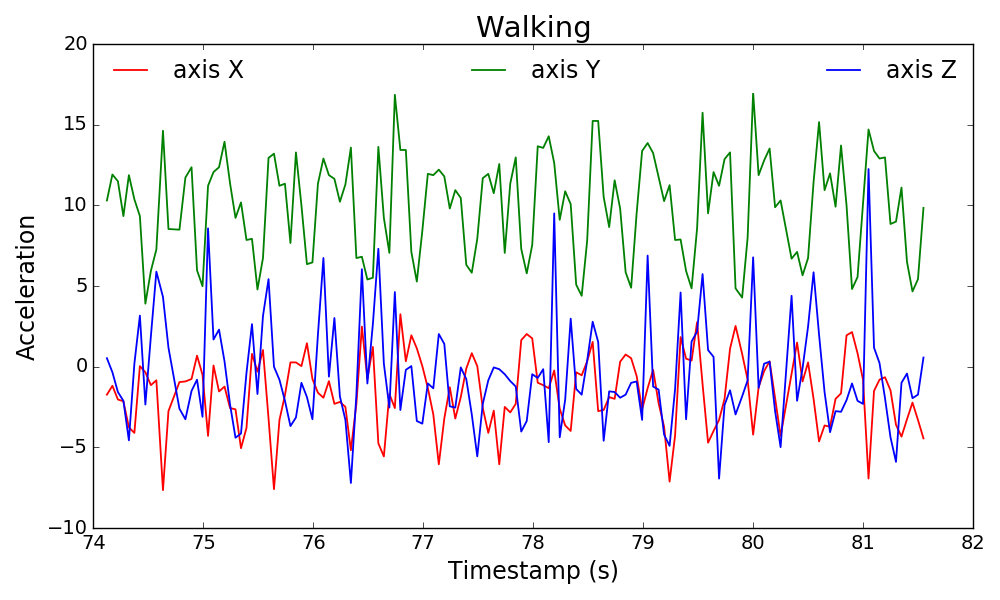
\includegraphics[width=1\linewidth]{ts_example.png}
	\caption{Time series example}
	\label{fig::ts_example}
\end{figure}

For each dataset apply feature generation procedures: expert functions, autoregressive model, SSA and splines. 
Three classification models for each generated feature description: logistic regression, support vector machine and random forest. 
The structure parameters: the length $n$ for autoregressive model, the window width $n$ for SSA and the number of splines knots $L$, were tuned using K-fold cross validation, minimizing
\begin{align}\label{cv}
CV(K) = \frac{1}{K}\sum_{k=1}^{K} L(f_k, \mathcal{D}\setminus \mathcal{C}_k),
\end{align}
where $C_k$ is a $\frac{K-1}{K}$ fraction of data, used for training model $f_k$.
The hyperparameters $\bm{\mu}$ for classification models were also tuned using the same cross validation procedure. 


The first approach for feature generation is expert functions. The main drawback of this approach is that we are restricted by our choice of the expert functions and these functions might be impossible to derive for some types of data.

The autoregressive model was tuned to find the optimal length $n$. Cross validation procedure gives optimal value $n=20$ for both dataset. 

The singular spectrum analysis was tuned in the same way to find the optimal window width $n$. Similar to autoregressive model, cross validation procedure gives the same value $n=20$.

We fit cubic splines~\cite{deboor1978splines} for time series using $scipy$ python library~\cite{scipy}. 
The knots $\{\xi_{\ell}\}_{\ell = 1}^M$ for splines were distributed uniformly. 
Value of~$M$ was chosen with cross-validation. 

The feature extraction methods gives the following number of features for both datasets: expert features: 40; autoregressive model: 63; singular spectrum analysis: 60; splines: 33.

The results of the experiments for the both datasets is presented in Fig.~\ref{fig::accuracy_results}. For WISDM dataset the worst result was obtained with spline approximation. 
The results for expert functions, autoregressive model and SSA is roughly identical. For USC-HAD dataset the results highly depend on the classification model. 
For both datasets logistic regression shows the worst quality, while the accuracy for support vector machine and random forest is almost the same.

\begin{figure}[!h]
	\centering
	\subfloat{
		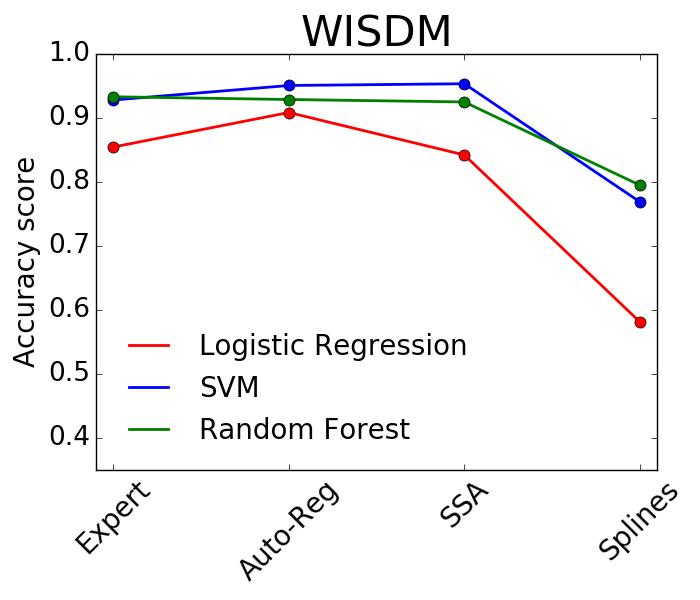
\includegraphics[width=0.49\linewidth]{wisdm_methods.png}}
	\subfloat{
		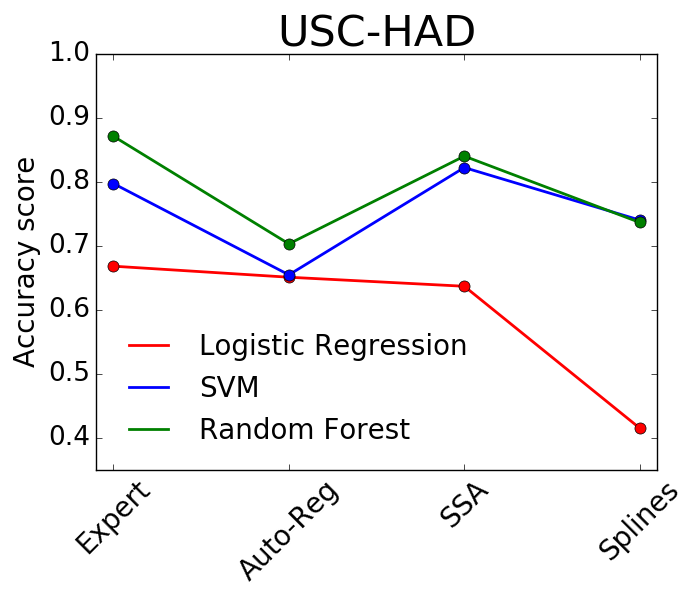
\includegraphics[width=0.49\linewidth]{uschad_methods.png}}
	\caption{Multiclass accuracy score}
	\label{fig::accuracy_results}
\end{figure}

All results with classification accuracy scores for each class are represented in Table~\ref{tbl::wisdm_methods_results} and Table~\ref{tbl::uschad_methods_results}. The first row of these tables introduces the multiclass accuracy score for each classification model and each feature extraction procedure. Next rows are related to binary accuracy scores for each class. For WISDM dataset the best scores have the least active classes such as Standing and Sitting. For USC-HAD dataset all classes have the similar accuracy scores.

\begin{table}[!h]
	\centering
	\caption{Binary accuracy scores for WISDM using different feature generation methods: EX~--- Expert, AR~--- Auto-Reg, SSA and  SPL for Splines}
	\footnotesize
	\begin{tabular}{r|rrrr|rrrr|rrrr|}
		& \multicolumn{4}{c|}{\textbf{Logistic Regression}} & \multicolumn{4}{c|}{\textbf{Random Forest}} & \multicolumn{4}{c|}{\textbf{SVM}}          \\ \cline{2-13} 
		& EX   & AR   & SSA   & SPL  & EX  & AR & SSA & SPL & EX & AR & SSA & SPL \\ \hline
		All& 0.85 & 0.91 & 0.84 & 0.58 & 0.93 & 0.93 & 0.92 & 0.79 & 0.93 & 0.95 & 0.95 & 0.77 \\
		Standing& 0.99 & 0.98 & 1.00 & 0.95 & 1.00 & 0.99 & 1.00 & 0.99 & 0.99 & 0.98 & 1.00 & 0.96 \\
		Walking& 0.91 & 0.96 & 0.86 & 0.61 & 0.96 & 0.97 & 0.95 & 0.86 & 0.96 & 0.98 & 0.98 & 0.84 \\
		Upstairs& 0.91 & 0.95 & 0.91 & 0.89 & 0.96 & 0.96 & 0.96 & 0.90 & 0.96 & 0.98 & 0.97 & 0.89 \\
		Sitting& 0.99 & 0.98 & 1.00 & 0.99 & 1.00 & 0.99 & 1.00 & 1.00 & 0.99 & 0.98 & 1.00 & 1.00 \\
		Jogging& 0.98 & 0.99 & 0.99 & 0.80 & 0.99 & 0.99 & 0.99 & 0.92 & 0.99 & 0.99 & 0.99 & 0.93 \\
		Downstairs& 0.93 & 0.96 & 0.94 & 0.92 & 0.96 & 0.97 & 0.96 & 0.92 & 0.96 & 0.98 & 0.97 & 0.92 \\ \hline
	\end{tabular}
	\label{tbl::wisdm_methods_results}
\end{table}

\begin{table}[!h]
	\centering
	\footnotesize
	\caption{Binary accuracy scores for USC-HAD using different feature generation methods: EX~--- Expert, AR~--- Auto-Reg, SSA and  SPL for Splines}
	\label{my-label}
	\begin{tabular}{r|rrrr|rrrr|rrrr|}
		& \multicolumn{4}{c|}{\textbf{Logistic Regression}} & \multicolumn{4}{c|}{\textbf{Random Forest}} & \multicolumn{4}{c|}{\textbf{SVM}}          \\ \cline{2-13} 
		& EX   & AR   & SSA   & SPL  & EX  & AR & SSA & SPL & EX & AR & SSA & SPL \\ \hline
		All& 0.67 & 0.65 & 0.64 & 0.41 & 0.87 & 0.70 & 0.84 & 0.74 & 0.80 & 0.65 & 0.82 & 0.74 \\
		Standing& 0.94 & 0.94 & 0.92 & 0.89 & 0.98 & 0.94 & 0.97 & 0.98 & 0.95 & 0.94 & 0.97 & 0.96 \\
		Elevator-up& 0.94 & 0.94 & 0.93 & 0.92 & 0.95 & 0.95 & 0.95 & 0.95 & 0.93 & 0.94 & 0.94 & 0.93 \\
		Walking-forward& 0.87 & 0.87 & 0.89 & 0.70 & 0.97 & 0.89 & 0.96 & 0.88 & 0.95 & 0.87 & 0.97 & 0.91 \\
		Sitting& 0.98 & 0.95 & 0.94 & 0.96 & 0.99 & 0.96 & 0.98 & 0.99 & 0.98 & 0.96 & 0.99 & 0.99 \\
		Walking-downstairs& 0.95 & 0.93 & 0.93 & 0.90 & 0.99 & 0.96 & 0.98 & 0.95 & 0.98 & 0.93 & 0.98 & 0.96 \\
		Sleeping& 1.00 & 0.98 & 0.99 & 1.00 & 1.00 & 0.98 & 1.00 & 1.00 & 1.00 & 0.98 & 1.00 & 1.00 \\
		Elevator-down& 0.94 & 0.94 & 0.94 & 0.91 & 0.95 & 0.95 & 0.95 & 0.95 & 0.93 & 0.94 & 0.94 & 0.93 \\
		Walking-upstairs& 0.94 & 0.95 & 0.93 & 0.92 & 0.98 & 0.95 & 0.98 & 0.96 & 0.98 & 0.95 & 0.98 & 0.96 \\
		Jumping& 0.99 & 0.99 & 1.00 & 0.97 & 1.00 & 0.99 & 1.00 & 0.99 & 1.00 & 0.99 & 0.97 & 0.99 \\
		Walking-right& 0.91 & 0.90 & 0.91 & 0.86 & 0.97 & 0.92 & 0.96 & 0.92 & 0.96 & 0.90 & 0.97 & 0.93 \\
		Walking-left& 0.89 & 0.91 & 0.90 & 0.88 & 0.97 & 0.93 & 0.97 & 0.93 & 0.95 & 0.91 & 0.97 & 0.93 \\
		Running& 0.99 & 0.99 & 0.99 & 0.92 & 1.00 & 0.99 & 1.00 & 0.97 & 1.00 & 1.00 & 0.95 & 0.98\\ \hline
	\end{tabular}
	\label{tbl::uschad_methods_results}
\end{table}

We also carried out the experiment for union of all $196$ generated features. The results are demonstrated on the Fig.~\ref{fig::feature_union_results}. In the Table~\ref{tbl::activities_distributions} one can see class labels, that are represented on the corresponding histograms. As expected, the accuracy scores in this case are higher in all cases. All binary accuracy scores for WISDM datasets is larger than $97 \%$ for each classification model. These numbers for USC-HAD dataset is larger than $93 \%$.

\begin{figure}[!ht]
	\centering
	\subfloat[WISDM dataset]{
		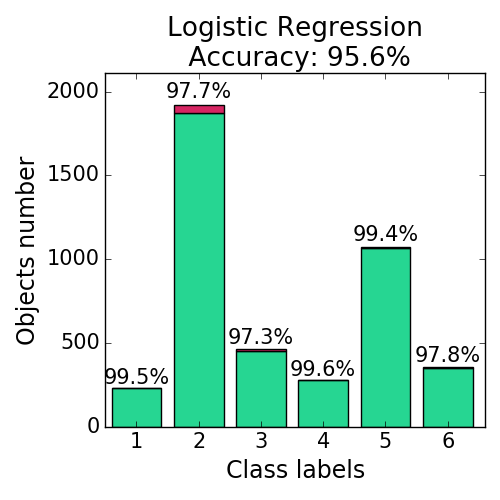
\includegraphics[width=0.33\linewidth]{pics/hist_wisdm_lr_all.png}}
	\subfloat[USC-HAD dataset]{
		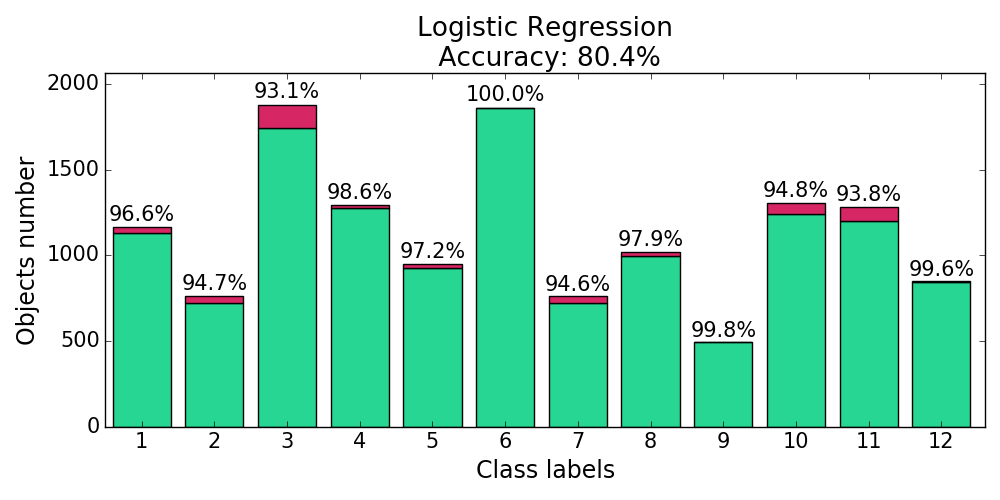
\includegraphics[width=0.66\linewidth]{pics/hist_uschad_lr_all.png}}\\
	\subfloat[WISDM dataset]{
		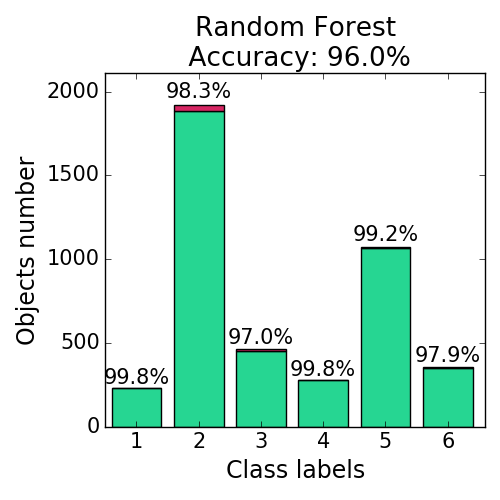
\includegraphics[width=0.33\linewidth]{pics/hist_wisdm_rf_all.png}}
	\subfloat[USC-HAD dataset]{
		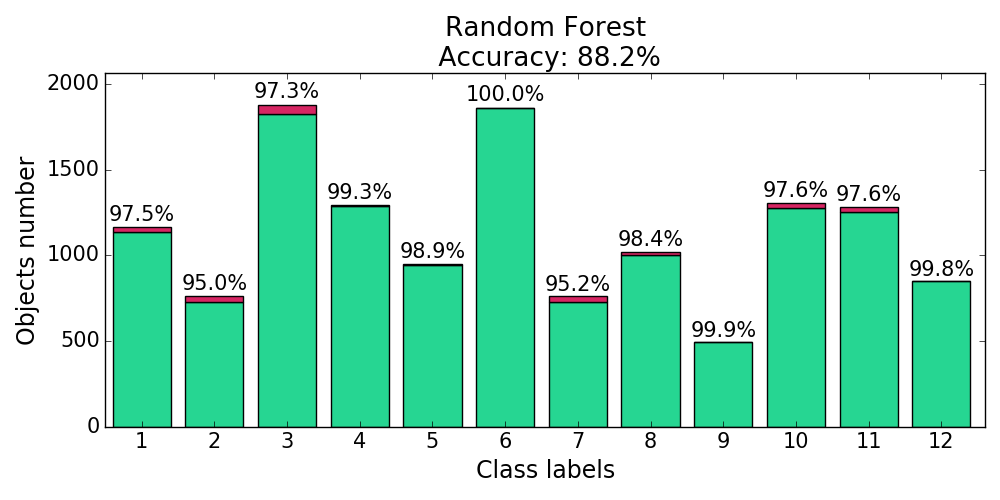
\includegraphics[width=0.66\linewidth]{pics/hist_uschad_rf_all.png}}\\
	\subfloat[WISDM dataset]{
		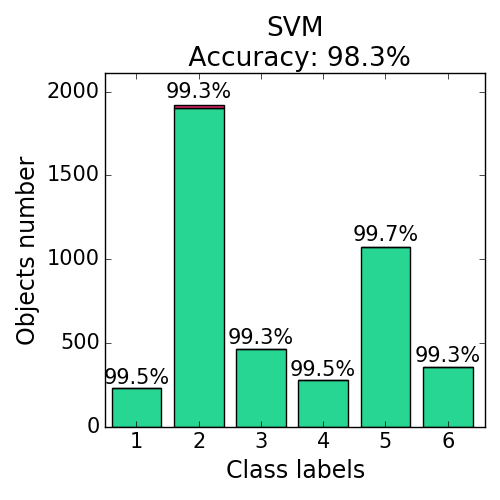
\includegraphics[width=0.33\linewidth]{pics/hist_wisdm_svm_all.png}}
	\subfloat[USC-HAD dataset]{
		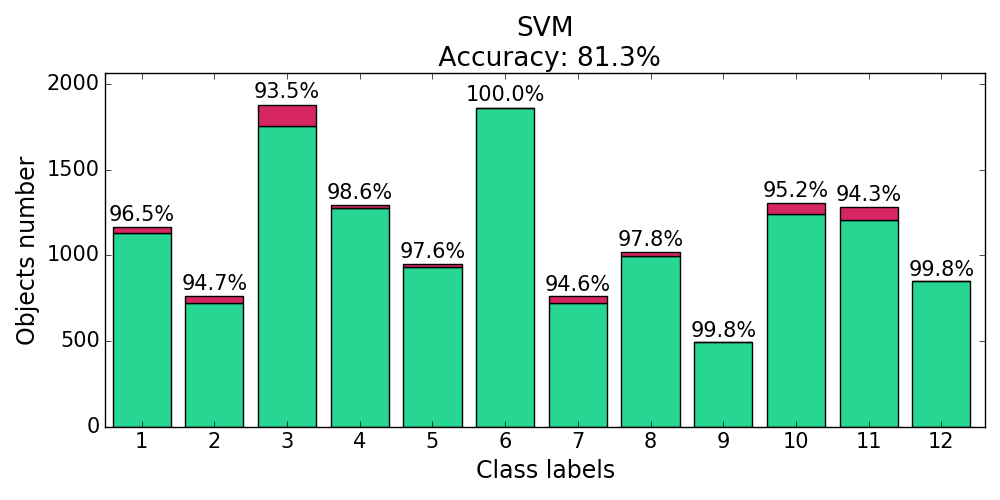
\includegraphics[width=0.66\linewidth]{pics/hist_uschad_svm_all.png}}\\
	\caption{Accuracy scores of classification of each class using all features}
	\label{fig::feature_union_results}
\end{figure}

\section{Conclusion}

The paper investigates the problem of complex structured objects classification.
The experiment compares various approaches of feature extraction, particularly the expert functions and local approximation models on data from smart phone accelerometer.
Logistic regression, SVM and random forest are used for classification. 
The results show that obtained features allows to recover the class label with the high quality.
\bibliographystyle{splncs03}

\begin{thebibliography}{10}
	\providecommand{\url}[1]{\texttt{#1}}
	\providecommand{\urlprefix}{URL }
	
	\bibitem{budnik2016learned}
	Budnik, M., Gutierrez-Gomez, E.L., Safadi, B., Pellerin, D., Qu{\'e}not, G.:
	Learned features versus engineered features for multimedia indexing.
	Multimedia Tools and Applications pp. 1--18 (2016)
	
	\bibitem{deboor1978splines}
	De~Boor, C., De~Boor, C., Math{\'e}maticien, E.U., De~Boor, C., De~Boor, C.: A
	practical guide to splines, vol.~27. Springer-Verlag New York (1978)
	
	\bibitem{geurts2001pattern}
	Geurts, P.: Pattern extraction for time series classification. In: European
	Conference on Principles of Data Mining and Knowledge Discovery. pp.
	115--127. Springer (2001)
	
	\bibitem{golub1970singular}
	Golub, G.H., Reinsch, C.: Singular value decomposition and least squares
	solutions. Numerische mathematik  14(5),  403--420 (1970)
	
	\bibitem{hammerla2016deep}
	Hammerla, N.Y., Halloran, S., Ploetz, T.: Deep, convolutional, and recurrent
	models for human activity recognition using wearables. arXiv preprint
	arXiv:1604.08880  (2016)
	
	\bibitem{hassani2007singular}
	Hassani, H.: Singular spectrum analysis: Methodology and comparison. Journal of
	Data Science  5,  239--257 (2007)
	
	\bibitem{ignatov2016human}
	Ignatov, A.D., Strijov, V.V.: Human activity recognition using quasiperiodic
	time series collected from a single tri-axial accelerometer. Multimedia tools
	and applications  75(12),  7257--7270 (2016)
	
	\bibitem{incel2013review}
	Incel, O.D., Kose, M., Ersoy, C.: A review and taxonomy of activity recognition
	on mobile phones. BioNanoScience  3(2),  145--171 (2013)
	
	\bibitem{scipy}
	Jones, E., Oliphant, T., Peterson, P., et~al.: {SciPy}: Open source scientific
	tools for {Python}. \url{http://www.scipy.org/} (2001--)
	
	\bibitem{karasikov2016feature}
	Karasikov, M., Strijov, V.: Feature-based time-series classification.
	Intelligence  24(1),  164--181 (2016)
	
	\bibitem{ivkin2015ts}
	Kuznetsov, M., N.P., I.: Time series classification algorithm using combined
	feature description. Machine Learning and Data Analysis  1(11),  1471--1483
	(2015)
	
	\bibitem{kwapisz2011activity}
	Kwapisz, J.R., Weiss, G.M., Moore, S.A.: Activity recognition using cell phone
	accelerometers. ACM SigKDD Explorations Newsletter  12(2),  74--82 (2011)
	
	\bibitem{lu2016activity}
	Lu, L., Qing-ling, C., Yi-Ju, Z.: Activity recognition in smart homes.
	Multimedia Tools and Applications pp. 1--18 (2016)
	
	\bibitem{lu2016towards}
	Lu, Y., Wei, Y., Liu, L., Zhong, J., Sun, L., Liu, Y.: Towards unsupervised
	physical activity recognition using smartphone accelerometers. Multimedia
	Tools and Applications  76(8)
	
	\bibitem{lukashin2003adaptive}
	Lukashin, Y.P.: Adaptive methods of short-term forecasting of time series. M.:
	Finance and statistics  (2003)
	
	\bibitem{umeda2017time}
	Umeda, Y.: Time series classification via topological data analysis.
	Transactions of the Japanese Society for Artificial Intelligence  32(3),
	D--G72\_1 (2017)
	
	\bibitem{usc}
	The usc human activity dataset.
	\url{http://www-scf.usc.edu/~mizhang/datasets.html}
	
	\bibitem{wang2014human}
	Wang, W., Liu, H., Yu, L., Sun, F.: Human activity recognition using smart
	phone embedded sensors: A linear dynamical systems method. In: Neural
	Networks (IJCNN), 2014 International Joint Conference on. pp. 1185--1190.
	IEEE (2014)
	
	\bibitem{wisdm}
	The wisdm dataset. \url{http://www.cis.fordham.edu/wisdm/dataset.php}
	
\end{thebibliography}

\end{document}